\documentclass{article} 
\usepackage[a4paper, margin=3.5cm]{geometry}

\usepackage{cite}

\usepackage{hyperref}

\usepackage{pgfgantt}
\usepackage{pdflscape}

\usepackage{tikz}

\usepackage{listings}
\usepackage[T1]{fontenc}
\lstset{basicstyle=\ttfamily}

\usepackage{tabularx}
\usepackage{colortbl}

\usepackage{graphicx}

\def\image#1#2#3#4{
	\begin{figure}
		\begin{center}
			\includegraphics[#2]{#1}
			\caption{#3}
			\label{#4}
		\end{center}
	\end{figure}
}

\def\imageh#1#2#3#4{
	\begin{figure}[h]
		\begin{center}
			\includegraphics[#2]{#1}
			\caption{#3}
			\label{#4}
		\end{center}
	\end{figure}
}

\title{\textbf{Influence Maximization Analysis. Progress Report}} 
\author{Antoni Zyla \and Supervised by Nathan Griffiths}
\date{}

\begin{document}

\maketitle
\linespread{1.25}

\tableofcontents

\newpage

\section{Introduction}

\subsection{What am I studying?}

Influence is the idea of a concept or idea spreading throughout a network.
It works well as a proxy for the spread of infectious diseases (SOURCE), behaviours (SOURCE) or even for helping with modelling physical processes (SOURCE CELF PAPER WATER LOSS)

Finding a subset $S$ of nodes from a network which have the greatest influence or spread is a well studied problem and there exist many models, algorithms and heuristics which help to efficiently achieve this goal.
This is an active area of research ... (SOURCE HERE)

\subsection{What do I hope to achieve?}
To find a heuristic which works well on a broad range of networks, performing better than others available for the same computing power or performing the same with less computing power.

\subsection{Why is this a good project?}

Systematic methods such as taking a greedy approach to find some set of influential nodes may seem like a good way to achieve a 'good enough' result.
Even a simple approximation such as greedy can take over 10 times longer than even an expensive heuristic approach whilst at the same time often producing a result less than or equal to the much heuristic method.

The performance of any method for determining the seeds is highly dependent on the network topology, size, and required $k$.
Being able to find a correlation between a topological property and an efficient seed selection method to produce high influences could allow for studies of (XXXX) to be made more efficient, more effective and (YYYY).
Study in this field is incredibly useful in working on social platforms, recommendation systems, trend analysis or network anaylsis to find emerging trends (SOURCE).


%Social networks \cite{sadasd}, interactions \cite{asdsad} and email chains \cite{enrondas} can all be modelled as a graph in the $G = (V,E)$ sense.

%Just as in a social setting concepts or ideas can spread through networks, for example if someone in a friend group takes up a new hobby then they have a higher chance of influencing their closest friends to try it than someone who they don't know.
%This idea leads directly into the independent cascade model (ICC), each node is able to infect every one of it's direct connections once with probability $p$.
%Those that it infects are then able to continue the cascade until there are no more active nodes.

%An extension of the ICC model is the decreasing cascade model (DCC), wherein the probability of a node being 'turned' by it's neighbors decreases each time it is attempted.
%If you see an advertisement for a certain product a very large amount of time you may be less likely to purchase or use the product due to overstauration/annoyyance.
%The rate at which we decrease the probability of infection is defined by a function $f(G, n) = p \in [0, 1]$.

%Another way of considering these problems is to consider a model where a node may adopt a concept after a certain proportion of it's neighbours have it.
%This models things such as immunity from diseases quite well.
%Each node is given it's own $t \in T$ where $T \sim  U(0, 1)$, once the node's proportion of infected neighbours reach $t$ then the node becomes infected.

%\subsection{Definitions}
%\begin{enumerate}
%	\item Let $G = (V,E)$ be a simple directed graph where $|V| = n$ and $|E| = m$
%	\item The graph is strongly connected; $\forall u, v \in V \hspace{0.5em} \exists (e_1, e_{2},..., e_{k})$ where $e_i = u$ and $e_k = v$ and $k \leq diam(G)$
%	\item $N(u) = |\{v \in V \hspace{0.5em} | \hspace{0.5em} (u,v) \in E \}|$
%	\item $diam(G)$ is the longest shortest path between any two nodes $u, v \in G$
%\end{enumerate}

%The report should be a self-contained document, so you should provide an introduction to the problem or area the work is addressing. You may wish to include some comments on your motivation for this such as the importance/timeliness of the investigation.

%You should include a copy of the original Project Specification as an appendix and can refer to this when appropriate.

%Make sure the objectives of your project are clear and clarify why this is a significant undertaking of suitable level for a third year project in your subject.

\section{Background Research}

I have considered a wide range of sources so far including research papers, doctoral theses, open source datasets, articles and open source code.
Each piece of information is cited and listed at the bottom of this document with as much information as I could include.

\subsection{Models of Influence Propogation}
There are three main models through which influence is typically spread across networks.

\begin{enumerate}
	\item Independent Cascade Model (ICC) - Each node can take a state out of Active, Inactive and uninfected (SOURCE).
	      Each active node has a probability $p$ to infect each of it's uninfected neighbors.
	      Once a node has been infected this process starts again to all of it's neighbors, the node is in the active state once it is infected (SOURCE).
	      Once a node has attempted to infect all of it's neighbors it becomes an inactive node.
	      This is the simplest of the models but also mimics real life very well, weather it's the spread of a new software technology or a new restaurant becoming more popular.
	\item Decreasing Cascade Model (DCC) - A modification of the ICC model where every attempt of a node to be influenced decreases the probability of it being influenced or infected. (SOURCE).
	      This is able to be modelled using a function $f: (v, n) \to [0, 1]$.
	      This could be analogous to a common experience, overreaching of advertisements or correspondence, such as marketing emails from the student union make me want to engage less with it due to being annoying and pushy.
	\item Linear Threshold Model (LTM) - Every node $v$ is given a probability of being turned $p$ which is uniformly distributed across the interval $[0, 1]$. When the proportion of node $v$'s neighbors which are infected is greater than or equal to $p$, $v$ itself becomes infected. (SOURCE)
	      This models well another common experience, a group reaching a common view in regards to something, whether it's the adoption of a new game, or even a software tool that becomes the 'industry standard' this principle is at play.
\end{enumerate}

As described above the independent cascade model is able to be easily modelled using the decreasing cascade model,
with the simple declaration of $\forall v \in V, f(v, n) = p, p \in [0, 1]$.

Working on the property of the expected influence as a fraction of nodes is a monotonic and submodular function of the number of seed nodes. (SOURCE)
\\

Various papers have described modifications of each of these models in a multitude of ways,
multiple concepts can be spread wherein they can inhibit the spread of eachother by allowing a node to only adopt a single concept (SOURCE).
Vaccination or heard immunity can be modelled in this manner (SOURCE).

There are other models which work in different manners, borrowing from biology models such as SI, SIS, SIR allow for modelling disease in a fine tuned manner (SOURCE). These are somewhat able to be modelled using the cascade models however full parity is not possible for example going from infected back to uninfected is not a behavior that is considered with the cascades and would possibly have large effects on the effectiveness of certain seed selection strategies (SOURCE).

There are models where paths between nodes can be added or removed as part of the process (SOURCE), this can for example be used to model the evolution of social networks, rather than studying networks which are at a fixed point in their evolution.
Similar cascade models can be used when studying these evolutions however this is an additional very large jump in complexity and scope which I would be unable to do in the time I have for this dissertation.

\subsubsection{Working with large networks}

Some of the networks I will be studying are made up of tens of thousands of nodes with hundreds of thousands of edges, working on networks of this size is almost impossible.
Most algorithms and processes are within polynomial time at the scale of the network they are not able to be feasibly used for most larger networks.

Sampling networks is a way of preserving the topological features and allows us to create strategies which generalise well to networks with a much greater size.

\subsubsection{Naive Approaches}
A simple natural approach could be to take a node at random from the graph, call it $v$, and then perform a breadth first search in layers across the graph.
A connected subset of size greater than or equal $k$ would be generated in $O(k)$, network topology is however unfortunately not well preserved.
When a high degree node is encountered then each of it's neighbours would also be added, this will inflate the average degree of the network by tending to sample a subset with a higher mean degree (SOURCE).

Working outwards from a start node in a layer by layer fashion does not preserve the distribution of shortest path distances between nodes well.
For node located close to the root these values will remain quite accurate but as we move further and further out a node is less likely to appear before we have no more nodes needed (SOURCE) leading to a lower shorter mean path lenght over the base network or other sampling methods.

Some papers describe BFS as adding the entire layer from which it explores, leading to oversized samples (SOURCE).
This is not useful when comparing like for like network sizes and their respective topological features such as diameter which are closely dependent on overall network size.
Snwoball sampling is a very simple variation on breadth first search,
once the addition of the final layer would take the total number of sampled nodes over the threshold, nodes are simply added one at a time until the exact number of nodes is reached.
In some networks taking a BFS sample of one thousand nodes may actually produce a sample of over twelve thousand nodes (REFERENCE Table somewhere below) which is in no way comparable to another methods 1000 node sample.
\\

A random walk is another simple strategy for exploring a graph.
Working on the basis of a standard random walk, starting from a node $v$ there is a $\frac{1}{deg(v)}$ probability of choosing the next node to be $u$ where $u$ is one of the neighbours of $v$.
Intuitively this helps with our shortcomings from BFS and SNS, the distribution of degrees would be more balanced as the probability of venturing to a low degree node is the same as to a higher degree one (SOURCE).

\subsubsection{Methods for finding seeds}
There are a few methods which don't rely on a heuristic to determine the seed nodes.

\begin{enumerate}
	\item Brute Force - there are n choose k possible seed sets from which to choose from.
	\item Greddy - Run a cascade from each node and then choose the $k$ highest influence nodes
	\item CELF - A modification of greedy which performs a little worse but is much much quicker at expense of lower overall efficacy.
\end{enumerate}

There are some approaches which I would like to consider that have been written about but not directly on the type of models that I am considering (INSERT INDIAN UNI PAPER + EXPLANATION).
\\

These approaches are a good estimation for the best possible result however are incredibly slow to run even on a modern processor.
Utilising a heursitic or approximation between a characteristic of a node and it's siginificance in spreading across the network can be a much more performant way of extracting similar results but at a computationally feasibly scale.

\textbf{TALK ABOUT THE HEURISTICS AND THE MAIN IDEAS AS TO WHY THEY WORK}

%You will have done a good deal of finding out about the project area by reading articles, books, websites, technical manuals and so on. You may have tested other related systems to provide ideas. You need to show that you have a good understanding of the background area and how your project fits into the existing landscape.


%There may be no room for a full literature review in the Progress Report, but you should give an indication of how you have gained background information. It would be appropriate to mention just a few citations which you view as key sources for your project. References should be provided as a formal reference list at the end of your report. Check if your supervisor has a preferred format. If not, you can choose your own style, but be consistent.

\section{Current Status}

Overall good progress has been made, a good portion of the desired objectives have been achieved.
The codebase is in average shape, documentation from docstrings is automatically generated into a navigable website that links between functions classes with examples of how use each function.

\begin{table}[h]
	\centering
	\begin{tabular}{|p{5.8cm}|p{2.9cm}|p{5cm}|}
		\hline
		\textbf{Objective}                     & \textbf{Status}    & \textbf{Notes}                                             \\
		\rowcolor{green}
		\hline
		1. Import and Export of Graphs         & Complete           & Not implemented unit testing                               \\
		\hline
		\rowcolor{green}
		2. Generation of Synthetic Graphs      & Complete           &                                                            \\
		\hline
		\rowcolor{green}
		3. Influence Models                    & Complete           &                                                            \\
		\hline
		\rowcolor{yellow}
		4. Sampling Methods                    & Partially Complete & TODO: Albatross Sampling                                   \\
		\hline
		\rowcolor{red}
		5a. Cost based analysis heuristics     & Incomplete         & Would be the most complex, may not implement if not needed \\
		\hline
		\rowcolor{green}
		5b. Minimum Nodes heuristics           & Complete           &                                                            \\
		\hline
		\rowcolor{green}
		5c. Rate vs Absolute change heuristics & Complete           &                                                            \\
		\hline
		\rowcolor{green}
		6. Packaging                           & Complete           &                                                            \\
		\hline
		\rowcolor{green}
		7. Parallelisation                     & Complete           &                                                            \\
		\hline
		\rowcolor{yellow}
		8. Documentation                       & Partially Complete &                                                            \\
		\hline
	\end{tabular}
	\caption{Current Status Summarised}
	\label{statusOverview}
\end{table}

Overall as from \ref{statusOverview} the project is in good shape to achieve all objectives by the end of term 2.

\subsection{Working with Networks}

As listed in objective \ref{objimportexport} my project needs the ability to import and export networks.
I have implemented the ability to import networks from a file as commonly found online \cite{}, custom delimiters are able to be used.
To make getting started with my program quick and easy I have included some networks inside of the python package, they are listed below in \ref{includedNets} along with some information about them.

\begin{table}[h]
	\centering
	\begin{tabular}{|c|c|c|c|c|c|c|}
		\hline
		\textbf{Name} & \textbf{Nodes} & \textbf{Edges} & \textbf{Mean Deg.} & \textbf{Cluster. Coef.} & \textbf{Diam.} & \textbf{Centralization} \\
		\hline
		Enron         & 36692          & 183831         & 10.020             & 0.497                   & 13             & 0.00725                 \\
		\hline
		P2P           & 10876          & 39994          & 7.355              & 0.006                   & 10             & 0.001899                \\
		\hline
		Airports      & 1574           & 17215          & 21.874             & 0.504                   & 8              & 0.004334                \\
		\hline
		Twitter       & 81306          & 1342310        & 33.019             & 0.565                   & 7              & 0.002114                \\
		\hline
	\end{tabular}
	\caption{Statistics on Included Networks with my package, to 3 d.p. when applicable.}
	\label{includedNets}
\end{table}

\begin{enumerate}
	\item \textbf{Enron} Email network from Enron an energy company that shut down in 2001 due to fraud (source needed).
	      Each email represents an edge, from the edgeset the network is then constructed (source of data).
	\item \textbf{P2P} Gnutella is a peer to peer (p2p) file sharing protocol created in 2000,
	      this network compiled in 2002 by (SOURCE) relates each host as a node and any connection between two hosts as an edge.
	      The protocol created some interesting topologies, with an overall goal of keeping the longest shortest path between any two nodes of at most 4 (source) it relied on a few nodes to act as an intermediate layer between the majority of clients. (MAYBE NOTE ON BEING SIMILAR TO KLEINBERG GRAPH WITH LEAFS ATTACHED)
	\item \textbf{Airports} A dataset of all flight traffic between american airports in 2010 (source tore opsahl).
	      This dataset is useful as due to the way it was gathered it will have likely a hub and spoke type topology due to the way airlines used to operate before small body airliners became commonplace (source needed).
	\item \textbf{Twitter} A large collection of circles, a feature which allowed users to specify to whom their tweets would go to, restricting these tweets from being public (SOURCE What is a Circle?).
	      It was obtained by crawling the website in 2012 by the Stanford SNAP research group (https://snap.stanford.edu/data/ego-Twitter.html).
\end{enumerate}

\subsection{Synthetic Networks}
Some papers (\cite{franks2014learning} and \cite{}) commonly compare synthetic networks to sampled networks from realworld structures.
As part of Objective \ref{objsynthetics} I have implemented the creation of both Kleinberg and Eppstein generators.
Examples of some networks produced by them are listed in the table below.

%\begin{table}[h]
%	\centering
%	\begin{tabular}{|c|c|c|c|c|c|c|}
%		\hline
%		\textbf{Name} & \textbf{Nodes} & \textbf{Edges} & \textbf{Mean Deg.} & \textbf{Clust. Coef.} & \textbf{Diam.} & \textbf{Centralization} \\
%		\hline
%		Kleinberg1000 & 961            & 4486           & 9.336              & 0.052                 & 14             & -0.0066                 \\
%		\hline
%		Kleinberg5000 & 4900           & 23390          & 9.547              & 0.0385                & 16             & -0.0013                 \\
%		\hline
%		Eppstein1000  &                &                &                    &                       &                &                         \\
%		\hline
%		Eppstein5000  &                &                &                    &                       &                &                         \\
%		\hline
%	\end{tabular}
%	\caption{Statistics on example synthetic networks with my package, to 3 d.p. when applicable.}
%	\label{syntheticGenerators}
%\end{table}

%The data in both table \ref{syntheticGenerators} and table \ref{includedNets} was easily generated in just a few lines of code and outputted a formatted table in the form of a pandas data frame as demonstrated below in the code for table \ref{syntheticGenerators}.


%\begin{lstlisting}[caption=Code to generate table \ref{syntheticGenerators}]
%nets = [
%    im.Network(name="Kleinberg1000"),
%    im.Network(name="Kleinberg5000"),
%    im.Network(name="Eppstein1000"),
%    im.Network(name="Eppstein5000"),
%]

%nets[0].kleinbergs_generator(1000)
%nets[1].kleinbergs_generator(5000)
%nets[2].eppstein_generator(1000)
%nets[3].eppstein_generator(5000)

%rows = [Metrics.generate_tabular_row(net) for net in nets]
%table = pd.concat(rows)
%\end{lstlisting}

\subsubsection{Navigable Small World Graphs}
\imageh{example_3by3_kleinberg_graph.png}{width=0.5\textwidth}{Example of a 3 by 3 Navigable Small World Network}{example_kleiberg_image}

A small world network is one that has a low mean shortest path between any two nodes and a high clustering coefficient.
This means that there is a high likelihood that any two nodes in the network are able to form a path between themselves using very few nodes, an example of this is the six degrees of separation theory.
\\

(NEED TO ADD SOURCE  J. Kleinberg, The Small-World Phenomenon: An Algorithmic Perspective, in Proc. 32nd ACM Symp. Theory of Comp., 163-170, 2000. )
\\

Table \ref{syntheticGenerators} shows the networks from the Kleinberg small world generator have an interesting pattern in regards to the number of nodes.
Both of the number of nodes are a square number, the networks constructed are $n \times n$ grids using the function within networkx, I did not implement an arbitrary $k$ node generator myself due to the additional time required, complexity and the likelihood of errors being introduced on my part.

\subsubsection{Power Law Degree Distrubted Graphs}

A power law graph means that the distribution of node degrees follows a power law distribution. (Source)
To form a graph with $k$ nodes a sequence of $k$ elements is created by sampling a power law distribution, the ability to form a graph from this sequence is then checked.
The graph is then initialised from a randomly generated graph with node degrees that follow this sequence.

\imageh{example_10_node_powerlaw_graph.png}{width=0.5\textwidth}{Example of a 10 node powerlaw graph}{example_eppstein_image}

This is an incredibly expensive process in terms of computation, generating a singe $k$ node graph is at minimum $O(k \log_2(k))$

\subsection{Cascade and Threshold Models}

As written in point \ref{objmodels}, Independent Cascade, Decreasing Cascade and Linear Threshold models have been implemented.
Code for automated running of trials, testing of heuristics on each of these has been written.
The required computations perform well when ran on the department's compute cluster.
Data is output in both tabular and graphical formats, below is an example of some early runs.

\image{../../results/early_hueristics_on_mhda_enron_2_sizes_all_models_abs_delta.png}{width=\textwidth}{Absolute Gains in Influence Compared}{earlyRuns}

\image{../../results/early_hueristics_on_mhda_enron_2_sizes_all_models.png}{width=\textwidth}{Early Running of Models with heuristics}{earlyRuns}

There are a few things we can garner from figure \ref{earlyRuns}:

\begin{enumerate}
	\item Degree based heuristics are very effective for how quick they are to compute.
	\item Clustering Coefficient is very effective, however only after a certain number of seeds, this could be due to how clustering and degree are presented, a high degree node may be connected to a significant proportion of the network whereas a node with a high clustering coefficient doesn't necessarily have a high possible number of effected neighbors.
	\item The asymptotic behavior of degree based heuristics is likely showing that the degree distribution of the network is one with a small number of very high degree nodes tightly packed. 
	Requring a large number of new seeds to make significant strides in terms of spread may show that high degree nodes are closely clustered together.
	\item There being minimal spread beyond the based starting nodes in the decreasing cascade and a convergence of the heuristics demonstrates that there may need to be some adjustment to the loss in turning a node per attempt.
	\item The linear threshold model shows a similar pattern to the independent cascade model with regards to there being two distinct groups of heursitics in terms of their results and behaviour at low seed sizes.
\end{enumerate}

\textbf{EXPAND ON ALL OF THIS AND MAKE IT SOUND NOT AWFUL}

Following figure \ref{earlyRuns} I implemented a few more heuristics as well as the naive greedy algorithm and the improved celf version.

\image{../../results/all_heuristics_icc.png}{width=\textwidth}{Currently Implemented Heurstics on ICC}{icc_all_heuristics}

\subsection{Evaluation of Sampling Methods}

As written in section \ref{probDiscSampling} of the specification, sampling methods 1 to 5 have been implemented.
Running multiple samples, collecting and collating the results has been written.
Tables similar to \ref{includedNets} or \ref{syntheticGenerators} are output with data about their mean and standard deviations.

\begin{table}[h]
	\centering
	\begin{tabular}{|c|c|c|c|c|c|c|}
		\hline
		\textbf{Method} & \textbf{Nodes}   & \textbf{Edges}     & \textbf{Mean Deg.} & \textbf{Cluster. Coef.} & \textbf{Centralization} & \textbf{Diam.} \\
		\hline
		Airports        & 1574             & 17215              & 21.874             & 0.504                   & 0.004334                & 8              \\
		\hline
		MHDA            & 1000             & 13585.60	 (301.08) & 27.17 (0.60)       & 0.498023 (0.006)        & -0.010 	0.0008          & 7.93 	0.25     \\
		\hline
		MHRW            & 1000             & 13575.87 (250.27)  & 27.15 	  (0.50)    & 0.50	(0.007)            & -0.010   0.0007         & 8.0 	0.0       \\
		\hline
		SNS             & 1000             & 15215.67	(312.83)  & 30.43 	  (0.63)    & 0.60 (0.02)             & -0.010 	0.001           & 4.47 	0.50     \\
		\hline
		BFS             & 1281.26 (132.39) & 16093.60  (652.30) & 25.30 (1.68)       & 0.55	(0.02)             & -0.0006	0.003           & 5.0	0.73       \\
		\hline
	\end{tabular}
	\caption{Various Sampling Methods on the Airports Dataset (15 Runs)}
	\label{enron_sample_methods_compared}
\end{table}

As shown in the above table \ref{enron_sample_methods_compared}; MHDA clearly shows that it is the closest method in terms of preserving the topology of the networks.

These results are also consistent with the data found in \cite{franks2014learning}.

In the project specification I outlined inclusion of Random Walk (RW) and Albatross (AS) sampling, I have not included those in this analysis as in comparison to MHDA there is little reason to use RW over the more advanced methods.

\subsection{Minimum Node Analysis}

%Sometimes you may want to find the minimum number of nodes $n$ such that for a given proportion $p \in [0,1]$ running the model with $n$ such seed nodes will produce at least $p$ infected nodes as a fraction of the total number of nodes.

%Calculating this could be done by running the cascade for $m$ nodes and then $m+1, m+2 ...$ nodes until the spread reaches the desired level.
%In terms of runtime this would be linear on |V| in terms of the number of cascade simulations.

%I took the approach of an exponentially increasing number of seeds $(1,2,4,8,16...)$ to find a pair of seed node sizes $(n_{under}, n_{over})$ such that they sandwich the target proportion.
%Utilising the fact that on average the influence spread is proportionally increasing with seed sizes, I can assume that the influence of models started with seed sizes along this interval will be sorted.
%This gives a maximum of $O(log|V|)$ cascades to find the 2 bounds and then $O(log\frac{1}{2}|V|)$ cascades to perform binary search along the $(n_{under}, n_{over})$ interval which has at most size $\frac{1}{2}|V|$.
%To further optimise the performance of this I added a parameter \texttt{quick} which allows for skipping of the secondary binary search procedure to give a rough estimate.

\textbf{INSERT GRAPH OF MINIMUM N's for heuristics and target proportion.}

Working out the minimum number of nodes for a given target proportion is simple if using a naive approach.
For a given network $G = (V,E)$ where $|V|=n$ and $|E|=m$ it would take $O(n)$ cascades to find such seed set size.

There is however a smarter and more efficient way of doing this computation.
Taking an ordered expnonetially increasing sequence of $S_n = (2^i, n)$ for $i \in \{0, 1, ..,  \lfloor \log_2{(n)} \rfloor  \}$ to denote the seed sizes we want to look at.
Noting that the sequeunce $S$ is of length at most $\log_2(n) + 1$.
Starting by iterating performing cascades from $S_1$ until we find $S_k$ where the influence spread of $S_k$ is greater than or equal to the required value.
As the influence is proprtional to a given seed set size and also increasing this implies that the influence of $S_{k-1}$ must be less than the required value.
Creating another ordered increasing sequence $A = (S_{k-1}, S_{k-1} + 1, ..., S_{k})$.
Noting that the sequence $A$ is of length at most $\frac{n}{2}$.
Performing binary search to the find the first element that is greater than or equal to the required value required taking $O(\log_2(\frac{n}{2}))$ cascades.
Combining both the large step and the small steps results in $O(\log(n))$ cascades being performed.
It may be easier to run binary search over the whole range $(0, 1, ..., n)$, the reason for going with the alternate approach described above is in the case of a low required target propogation.

On a large network the cascades are a costly computation, some networks with high degree values can achieve almost $\frac{1}{3}$ of their total nodes infected by a single seed node.
Iterating upwards turns this into a very quick computation rather than performing $\log(n)$ costly cascades to just find the first element.


\subsection{Rate of Change Analysis}

Running each of the models returns a triplet of the number of iterations, the final influenced graph, and an array of influenced proportion values $\in [0, 1]$ of length of the number of iterations.

The data produced here mirrors the behaviour exhibited in some of the other graphs. In effect an iteration of a quickly spreading graph is just introducing more seeds so the behaviour should mimick that of the overall growth graphs.

\textbf{INSERT TABLE OR GRAPH DEMONSTRATING THIS EFFECT}

\subsection{Packaging}

I am utilising an open source python library packaging tool called Hatchling, allowing me to package the entirety of the code into a \texttt{.tar.gz} and a \texttt{.whl} distributable.
Python3.10 and above is required due to the introduction of union types in the type annotation system.
I have attempted to use PyPy (the JIT compiling interpreter) however there were some issues with the multiprocessing code so I have decided to not focus on this aspect.

%Installing and running the code is simple on any environment with an installation of python 3.10 or newer as shown in the below snippet.

%\begin{lstlisting}[caption=Utilising my code]
%shell> pip install Influence_Modelling.whl 
%
%from Infleunce_Modelling import Network as im 
%import networkx as nx
%
%net = im.Network("test-network")
%net.set_nx(nx.complete_graph(10))
%iters, final = net.run_icc()
%\end{lstlisting}

\subsection{Parallelisation and Performance}

Performing hundreds of cascade processes on tens of networks on tens of sample methods with tens of different seed sizes requires a large amount of computation.

Utilising the multiprocessing module in python it was relatively simple to implement multiprocessing in my testing and data generation scripts.
Each task such as run a cascade on this network with this sampling method with this many seeds using this heuristic is created as a tuple of inputs into an array, using the \texttt{Pool.starmap} function it's easy to perform a catchall function on these and get the results using an arbitrary number of threads to complete the processing.

One of the main challenges with regards to running these processes quickly is sampling of large scale networks, sample methods such as MHDA require a large amount of computation steps for each node that is added and each of these steps are at least linear with the size of the network.

Saving a set of previously sampled networks and then running cascades on each of them is a simple way to make the overall performance of generating results much quicker.
\\

When working in this manner performance is hugely increased, this will allow me to generate results much quicker and give a quicker feedback cycle of testing ideas from conception to results. 
\textbf{INSERT A TABLE OF THIS ACTUALLY MAKING A DIFFERENCE}

%Running trials and generating samples of networks has been implemented using pools and python's multiprocessing library.
%Performance is good when it's shared across a single node, splitting across multiple physical servers resulted in a minor speedup at the expense of much higher communication cost.
%This is not a large problem as I can split my running of the testing into sepearate invocations of my scripts on the different nodes.

\subsection{Documentation}

JavaDocs style documentation is automatically generated on every commit using GitHub actions to run a CI pipeline.
Key information is taken from docstrings enclosed by a triple set of inverted commas, detailing information such as what the function does, example usage, input and return types.

A fully searchable and navigable set of static web pages is generated, in the future this could be embedded within a wider set of documentation including systems design, user guides, troubleshooting guides and various other resources.

%As part of the projects packaging phase automatic documentation is generated from the usage of python docstrings, this is done using an opensource library called pdoc \footnote{https://pdoc.dev/}.
%Using github actions this build steps runs on every commit to the main branch of the repository and this generates a navigable and searchable documentation base as shown in figure \ref{pdoc-example-screenshot}.

\image{example-pdoc-documentation.png}{width=\textwidth}{Example of automated documentation site}{pdoc-example-screenshot}

%Provide an overview of your work so far. This should include:

%Technical Content - what work have you done? You should provide a meaningful discussion of the significant aspects rather than simply saying "I did x, y and z". This is necessary to show you've actually done it and in order for your assessor to award marks according to the assessment criteria.

%Progress - review your progress against the original timetable. If unexpected problems or delays have occurred, how have you dealt with the problem?

\subsection{Technical Content}
Talk about code structure, data collection, processing of data, saving intermediate steps in all computations, using the hpc cluster, typical performance of runs.

\subsubsection{Code Structure}

The primary code is structured in an object oriented fashion, for example a network is a class which is then extended into a network that reads or writes csv files.

Each of various sections I need to use are split into multiple files and these all have to be imported separately when being used.

Most of the code is used in interactive notebook environments.

My test scripts are standalone scripts that simply require the packaged library to be installed alongside some other libraries, these are the scripts which produce the results as displayed in all the tables and figures so far in this document.

\textbf{INSERT UML OR SIMILAR DIAGRAM}

\subsection{Performance}

For every run of a cascade, sampling method or any action I record the time taken, if running over a large number of samples I also automatically take the mean and standard deviation of the running time and this is an extra column at the end of each of the tabular outputs for any aggregate process.

This quite clearly shows how a more complex heuristic can be over a hundred times slower than a simple one like degree, with the greedy algorithm and celf being hundreds of times slower than even the slower heuristic.

\textbf{INSERT BAR CHART COMPARING PERFORMANCE BETWEEN DIFFERENT METHODS}

\subsection{Data Visualisation}

Something that is not immediately clear is how to best present data to easily and accessibly show the results and conclusions I am trying to make. I did not set out any clear requirements for this as at the time of writing the specification I did not yet know the best ways of presenting data and what ways would be most relevant to my results.

Showing a busy graph with lots of lines may be good for a vague overview or rough ordering of performance characteristics of each heuristic but it is not very useful for detailed close comparisons.
\\

Following on advice from my supervisor I am in the process of implementing more intuitive visualisations. 
So far I have the following.

\textbf{ADD EXPLANATION FOR EACH OF THOSE BELOW}
\begin{enumerate}
	\item Total spread for each seed size and heuristics
	\item Absolute gain in influence for seed size and heuristics
	\item Tabular network data Statistics
	\item Tabular total influence spread for each seed size and heuristics
	\item Offset spread graphs using one of the lines as new 0 line and giving the others as above or below to show relative orderings.
\end{enumerate}

\textbf{LIST OF NEW WAYS I WILL DEMONSTRATE AND SHOW DATA }

\section{Upcoming Goals}

Talk about being on track with the goals from the gannt chart in spec, need to implement some more stuff and actually do some independent testing and evaluation of my own ideas.

\textbf{INSERT NEW GANT CHART MODIFIED WITH WHAT HAVE LEARNT SO FAR}

\subsection{Areas I will Investigate}

An iterative approach based on a combination of greedy and heuristic methods.
For example choose seeds by degree, redo degree but don't include any nodes that that node has spread to over a few iterations of the cascade model.
Similar methods have been described in some papers (SOURCE) but working on a different model with a much different set of comparison methods.

%You may have changed your plans for the remainder of the project. 
%At the very least, you are likely to have a much clearer idea of how things will proceed and the timings needed to complete each stage.

%Outline your plans for the remainder of your work on the project, and any alterations to your original ideas.

%Provide an updated timetable with as much detail as possible.

\section{Reflection}
%What is your assessment on how things have gone so far
In terms of the technical goals the project is doing quite well.
Most functions are complete and work as intended, results are able to be generated and presented in graph or tabular form quite quickly and efficiently.

I am concerned about my ability to actually create a new heuristic which will outperform those which have already been studied.
I have explored some ideas regarding taking combinations of nodes that are both in a large cluster as well as those with a high betweeneess, the results seem to be very network topology dependent creating a large variance in performance of the same algorithms with the difference stemming from individual network and sample variances.
Further study in all areas of this will be required and a deep analysis behind the why of this behaviour is found.
\\

Primarily in and around the middle of the first term I started to focus on my graduate job search which not only took a lot of time but also made me quite demotivated in general.
I find that when I have a new task to focus on I will hyper focus on that task and disregard my other obligations.

%Are there lessons learned that you can use to make the work run more smoothly during your remaining work on the project?

\section{Project Management}

%How have you managed the project so far? You may be using a formal methodology (e.g. for software development or management of code versions). It may also be appropriate to refer to less formal ways of keeping on track, for example, regular timetable reviews with your supervisor.
Progress is on track with what I specified in the specification.
The gantt chart was relatively close to what happened and required little changes.

All code versions, results and documentation are held in a git repository.
This is stored with a main repository stored by GitHub with my personal computer and the DCS lab machines holding up to date copies as I work on them.

Keeping track of tasks and goals for the immediate terms was quite difficult for me.
I primarily kept track via a simple list in my notebook and by adding entries to my google calendar.



\section{Legal, Social, Ethical and Professional Considerations}

As per section \ref{lsep} of the specification there have been no changes to this.
% this removes the spec to check word count
% \end{document}

\newpage

\appendix

\section*{Appendix: Project Specification}
\section{Abstract} \label{abstract}

A network is a weakly connected directed graph about which we reason.
Influence is the measure of how ideas or properties spread through this graph based on certain models;
choosing the seed set of nodes from which to begin the model determines how quickly and how far the ideas will propagate.
Social networks \cite{yang2019influence}, infectious diseases and behaviors \cite{archbold2024cvd} can be studied by using such an approach and can be used to inform decision making in many areas.

Finding a subset of nodes of the network which produce the greatest influence spread after a given time period could be used to determine those who'd best promote a product or be at greatest risk of spreading an infectious disease \cite{archbold2024cvd}.
Finding this subset is difficult and known to be NP-Hard, as a reduction from Vertex Cover \cite{kempe2005influential}.
Using certain heuristics such as the degree of a node to choose the seed nodes is significantly more efficient running in polynomial time \cite{chen2009efficient}.

Using real world networks to perform this analysis on is not only difficult to obtain but also very large and computationally intensive \cite{Wang2011UnderstandingGS}.
I will aim to create a tool which can be used to evaluate and compare different heuristics and sampling methodologies against different types of networks.
I will then use this tool to find a more representative sampling method on networks, or a heuristic which works more effectively on a certain set of topologies.

\section{Problem Discussion} \label{probDiscussion}

I will define a network upon which the models below will work on as a weakly connected directed graph.
Doing so allows for modelling of networks in which the relationships are bidirectional (undirected) by simply creating two edges to represent that relationship, and for modelling directed networks such as email chains that have a clear sender and recipient.
To be used for analysis, the network needs to be connected, as an idea cannot directly propagate between two disjoint components.

\subsection{Models} \label{probDiscModels}
\begin{enumerate}
	\item Independent Cascade Model (ICM) - a node can be 'active' or 'inactive' and has a constant probability of infecting each of it's neighbours.
	      Every infectious node has one attempt to infect it's neighbours before becoming inactive \cite{kempe2005influential}.
	\item Decreasing Cascade Model (DCM) - an extension of the IC model the probability of infecting a node is determined by previous attempts, modelling how subsequent attempts are less likely to be successful after failed attempts \cite{kempe2006influential}.
	\item Linear Threshold Model (LTM) - A model where each node has a certain 'threshold' required to infect it, considering the cumulative effect of the already infected nodes on the node determines if it will become infected \cite{kempe2005influential}.
\end{enumerate}

\subsection{Sampling Methods} \label{probDiscSampling}

Some real world datasets are far too large to efficiently compute these models on.
Sampling these networks allows us to find a smaller network that encapsulates their features but is much more efficient to perform computations on.
Those listed below I have researched and feel would be able to implement and use to evaluate against one another, as research progresses I may choose to add more methods or to not use a certain method.

\begin{enumerate}
	\item Breadth First Search (BFS) - A natural exploration of the graph from a random node in layers \cite{franks2014learning}.
	\item Snowball Sample (SNS) - An extension of BFS which will stop once the desired sample size is reached \cite{franks2014learning}.
	\item Random Walk (RW) - Starting at a random node in the network chooses where to go onwards based on the the node's neighbours being chosen at random.
	\item Metropolis Hastings Random Walk (MHRW) - A random walk with a modification to the probability function used to determine the subsequent node. This is to generate a uniform distribution of node degrees by favouring lower degree nodes \cite{gjoka11practicalreco}.
	\item Metropolis Hastings Random Walk with Delayed Acceptance (MHDA) - A further modification of MHRW in which the probability of backtracking to the previous node is reduced \cite{lee2012randomwalkmetropolishastingssamplers}.
	\item Albatross Sampling (AS) - A random walk with a chance of jumping to other locations in the network to find connected components \cite{jin2011albatross}.
\end{enumerate}

\subsection{Heuristics} \label{probDiscHeuristics}

Choosing which nodes to start the models on will affect how quickly the influence will propagate and how far it will spread to.
A greedy approach may be close to optimal, however on larger datasets is inefficient and potentially intractable \cite{griffiths17LimitiingConcept}.
The following are some of the methods by which I will investigate, during the research phase I may add more or I may exclude some.

\begin{enumerate}
	\item Random - As a baseline choose $k$ random nodes.
	\item Degree - Choose nodes with the highest degree.
	\item Degree Discount - A modification of the degree heuristic but with a lower chance of choosing a node if it's neighbour is in the seed set \cite{chen2009efficient}.
	\item Local Clustering Coefficient - The extent to which neighbours are connected to one another \cite{franks2014learning}.
	\item Average Neighbour Degree - Measuring the average degree of a node's neighbours may allow for communicating with high influence nodes \cite{franks2014learning}.
	\item Betweenness Centrality - Measuring how many shortests path's in the network pass throuhg a point \cite{franks2014learning}.
	\item Average Shortest Path Length - A measure of centrality by taking the mean length of the shortest path from the node to every other node \cite{franks2014learning}.
	\item Edge Embeddedness - For an edge $(u,v)$ is the size of the intersection of the neighbourhoods of both $u$ and $v$ \cite{franks2014learning}. This serves as a measure of how tightly packed a network is around a certain area.
	\item Edge Overlap - For an edge $(u,v)$ the edge overlap is the ratio of it's embeddedness to the size of the union of the neighbourhoods of $u$ and $v$. This can be used to determine the 'location' of an edge, for example if it connects connected components it may have a low overlap whilst a very high embeddedness may indicate not only is the agent well connected inside it's cluster it's also connected to other clusters \cite{franks2014learning}.
	      % \item Maximum Probable Gain - Used in research about spreading an inhibiting concept (against a target concept in ICMs) by choosing nodes with a high expected number of activations for the target concept \cite{griffiths17LimitiingConcept}.
	\item Traditional Greedy Algorithm (Select Top $k$ in \cite{yang2019influence}) - Choose greedily from nodes which have the highest influence \cite{kempe2005influential}. This is inefficient due to requiring running a cascade for each node. It approaches within $(1-1/e)$ of the optimal solution so will be used to compare against heuristics.
\end{enumerate}

\subsection{Application to research} \label{implementation}
Utilising the above concepts, possible pieces of research in this area may include:
\begin{itemize}
	\item Finding a more effective or representative heuristic for finding seed nodes in a network.
	\item Optimising a heuristic's running time whilst maintaining performance in regards to representation.
	\item Finding a more representative sampling method for varied network topologies.
	\item Finding a correlation between certain topological features and the effectiveness of one sampling method or heuristic over another, particularly in relation to that network feature.
\end{itemize}

\section{Objectives} \label{objectives}

The exact goal of my project is not fully decided, however there are some requirements for the code.
With these features I would be able to perform much of the computation and comparison of various papers.
Ideally I would be able to find something new or improve on existing techniques as described in section \ref{implementation}.

\begin{enumerate}
	\item Facilitate import and export of different graph formats. \label{objimportexport}
	\item Generation of synthetic graphs using graph generators for consistent analysis when real world datasets could be too large to run quick computations on. \label{objsynthetics}
	\item Running and evaluation of the Independent Cascade Model, Decreasing Cascade Model and  Linear Threshold Model. \label{objmodels}
	      Allowing for evaluation of different heuristics against these models on different graphs.
	\item Creation and evaluation of new sampling methods. \label{objNewSampling}
	      \begin{itemize}
		      \item Evaluate the running time of sampling algorithms in practice, finding the real world constant factors.
		      \item Allow for evaluation of influence spread on the same network with different samples and how they affect it.
	      \end{itemize}
	\item Creation and evaluation of new heuristics for selection of seed nodes against benchmark algorithms.
	      \begin{itemize}
		      \item A 'cost' based strategy could be to give each algorithm a total cost, and each node has a value with the aim to find the subset that produces the greatest spread from nodes within a certain total 'cost'.
		      \item	A 'minimum nodes' strategy to meet some spread metric, for example finding the lowest number of nodes that will produce a $\delta$\% spread after $x$ iterations.
		      \item Investigation of heuristics focused on overall growth in influence or rate of change in influence - this would involve charting the growth rate of various heuristics against eachother with trendlines etc.
	      \end{itemize}
	\item Python \textbf{whl} and \textbf{tarball} packaging to allow for easy installation on various systems.
	\item Programming with parallelisation in mind.
	      Some results may take hours to compute on a personal device but are able to be ran in parallel on a cluster or more powerful system.
	      I will attempt to use the batch compute system to produce any results.
	\item Fully document all code, usage examples, parallelisation examples, and everything required to produce any results in my final report.
\end{enumerate}

\section{Methods and Methodology} \label{methods}
%How are you going to approach your project?
% If system development is required, how will you be managing that?
% Is it appropriate to apply an accepted development methodology? 
%If so, which one? If not, how are you approaching the development? 
%If you're investigating a business topic, what methods will you be using? 
%Common ones might be literature review, case study, survey and interview. If you're conducting a survey, are you aware of good survey design? If you're planning interviews, what methodology will you use to analyse and represent the responses? 
%Whatever the nature of your project - what methods are you using to ensure that it stays on track and achieves its goals?

The project will be broken up into three main stages; research, implementation, and evaluation.
During each stage I will be in contact with my supervisor to ensure that I am on the right track and to keep me accountable.

\begin{enumerate}

	\item The research stage will require a detailed literature review of articles and papers pertaining to network influence modelling, methods, heuristics and sampling.
	      I will identify the validity and applications of each source and find whether there are any gaps in the presented knowledge to research further.
	      I will repeat this process until my supervisor and I are happy the full scope of the project has been thoroughly reviewed.

	\item The implementation stage of the project will require a methodology that can be adapted to changing requirements or a shift in focus based on information learnt in the later stages of the research phase.
	      I will use an agile-like methodology, of one to two week sprints determined by meetings with my supervisor, with any changes to requirements determined during these meetings with future sprints based on the previous.

	\item I will use my framework to replicate the results of the researched papers, showcasing how to create new sampling methods and heuristics, and how to compare the results of different sampling, heuristics and models on different networks.

	\item Finally, I will attempt to improve upon a sampling method or heuristic and use my framework to do so. This will demonstrate that my tool is applicable to real world research uses and potentially find something interesting or noteworthy.

\end{enumerate}


\section{Timeline} \label{timeline}

The schedule is not fully decided at this point as the research phase is yet to be completed and the further points maybe change.
Some points such as writing the report in the month leading to the deadline are certain, however the contents and direction of that report is not yet concrete.
The purple bars on the gantt chart are the deliverables and the yellow bars are the main sub-tasks associated with those deliverables.

\begin{figure}[h]
	\centering
	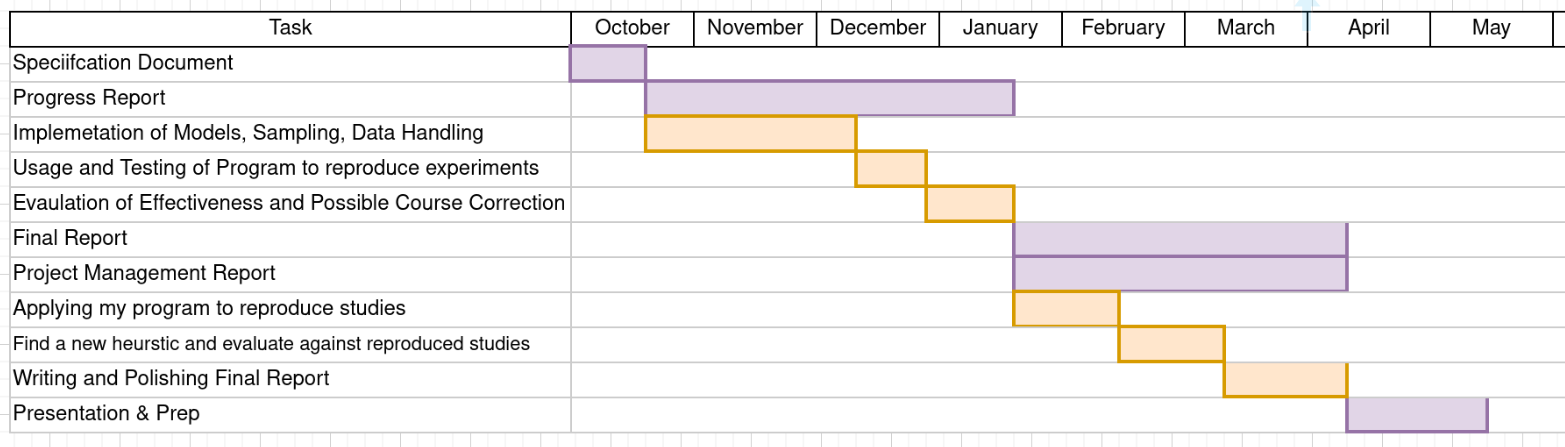
\includegraphics[width=\textwidth]{../../images/9octGanntChart.png}
	\caption{Gantt Chart of Expected Timeline}
\end{figure}

\section{Resources and Risks} \label{risks}

%%What resources does your project rely on? 
%For example, the list might include the hardware to be used, any non-standard software, data that a company has promised to provide or even subjects to take part in an interview. 
%Have you thought about what would happen if any of these resources became unavailable? What is your back-up plan? 
%This part of the Project Specification should show that you've thought these issues through and that you have appropriate back-up plans in place where necessary. 
%For more discussion on resources and managing risk, check out the information on equipment and other resources.

\subsection{Resources} \label{resources}
\begin{enumerate}
	\item Python and Standard Libraries - NetworkX, NumPy, Pandas, Matplotlib, Build tools.
	      These are all commonly available on a variety of systems, are open source, and can be built from source in case PyPI is unavailable.

	\item Large Graph Datasets - Enron emails, airport traffic data, Gnutella data, Twitter tweet data and any other data sets as research progresses.
	      The data is available from multiple sources on the internet, as well as being stored in the repository of my program under version control.

	\item Batch Compute System - Department of Computer Science (DCS).
	      The datasets I will be working with are large but not unmanageable on a typical desktop.
	      The batch compute system will be used to learn and utilise good practice for scientific computing, as well as allowing for faster computation.
\end{enumerate}

\subsection{Risks} \label{riskDetails}
\begin{enumerate}
	\item Failure to find a new heuristic or sampling method that is measurably better than those currently written about.
	      In this case the project would still be a success as it would show that it allows for evaluation of heuristics effectively to be able to show that it is not statistically better.

	\item Lost or damaged device containing code and documents.
	      Using GitHub to be a remote mirror of local git repository and regularly committing code will prevent issues from lost work arising.
	      DCS machines are more than adequate for processing needs.
\end{enumerate}

\section{Legal, Social, Ethical and Professional Considerations} \label{lsep}

At this stage there are no legal, social, ethical or professional considerations to take into account.
The project will not be using, processing or interacting with personal data or information.

\newpage
%\nocite{*}
\bibliographystyle{abbrv}
\bibliography{../sources}{}

\end{document}
